\section{Process' Perspective}
% In essence it has to be clear how code or other artifacts come from idea into the running system and everything that happens on the way.


\subsection{Team Interaction and Organization}
% How do you interact as developers?
% How is the team organized?
% Danyal

\subsubsection{Meeting times}
The way we worked is that we treated each week as a "sprint" where we would mainly work asynchronously. Once per week, 3 hours before the lecture would start, we would meet up at ITU to synchronize on work that had been done from last week and assign new tasks. We kept this going consistently throughout the whole course with few exceptions, such as in times where workload would be especially high.\newline
The mediums used for interaction was:
\begin{itemize}
    \item Discord server - messages and voice calls
    \item Weekly in-person meetings at ITU
    \item GitHub project board for organizing tasks/issues
\end{itemize}

\subsubsection{Work delegation}
Tasks would be created from users, taken from weekly course tasks, or created internally based on status of implementing different tools or functionality.\newline
As all of us were new to the concepts introduced throughout the course, we weren't able to pair up someone experienced with someone inexperienced, which would have been the ideal scenario for us. Therefore, we would typically try to assign 2 people, but as technical debt began piling up, we sometimes had to assign 1 person to a tasks, which was not ideal. 

\subsection{Description of Stages and Tools Included In the CI/CD Chains}
% A complete description of stages and tools included in the CI/CD chains.
% That is, including deployment and release of your systems.
% adam
Git version control, hosted on github.
Repository setup and branching
Kanban
Docker-compose file

Digital Ocean as IaaS vendor.


\subsection{Organization of Our Repository}
% That is, either the structure of of mono-repository or organization of artifacts across repositories.
% In essence, it has to be be clear what is stored where and why.
% Danyal
The way our repository is set up is that we have one repository with all of our services. We had some issues with folder structure in the beginning, but managed to figure a structure out that worked nicely for us. As most of our services are containerised and the specification for the service is defined within our docker-compose.yml file, we had no issues with identifying where a specific service would be.


\subsection{Applied Branching Strategy}
% Danyal
For this project we decided to go with two standard branches, one for each environment; \textbf{development} for the development environment and \textbf{main} for the production environment.

The \textbf{development} branch is for testing our code. Here is where every newly developed feature is merged into as per default when creating a pull requests. This is also where we would discover if any new features were to introduce unforeseen bugs. It is also the branch that every new feature should branch out of.

The \textbf{main} branch is our production environment. This is our "live" code and is what the current state of our product looks like. This is also to define what is ready to use for our users.

Whenever a new feature is to be initiated, this should happen in a new branch. This new branch should be named after the new feature. Following this naming convention allows other developers to keep a track of what each branch is for.

This was all agreed on internally, but later decided needed to be set in stone and so the "CONTRIBUTING.md" file was pulled in to our repository.


\subsubsection{Development Process and Tools}
% For example, how did you use issues, Kanban boards, etc. to organize open tasks
% Sabrina

Our team used a variety of software development tools and methodologies to ensure efficient collaboration, project organisation, and task tracking.

\subsubsection*{GitHub Issues and Projects}

We used GitHub Issues to record and track all tasks, improvements, and bugs associated with our project. This made it easier for our group to keep track of what needed to be done, as well as assign tasks to each person. We set up a Kanban board within GitHub Projects where we kept the backlog of all issues and their current state. The states we defined are as follows: 
\begin{description}
    \item[\textbf{New}] Tasks identified but not fully defined or prioritized.
    \item[\textbf{Ready}] Tasks with clear acceptance criteria and ready to be worked on.
    \item[\textbf{In Progress}] Tasks under active development.
    \item[\textbf{Review}] Completed tasks to be reviewed by another developer.
    \item[\textbf{Done}] Tasks that have passed all acceptance criteria.
\end{description}

This system made it easier for us to keep track of which stage each task was at and as serving as a visual cue of our workload.

\subsubsection*{Discord}

Discord was our chosen platform for remote communication. We used it for pair-programming collaboration, helping each other when we had any issues and planning next steps. 

We found that these tools helped us maintain transparency, encouraged collaboration, and ensured that every team member was kept in the loop regarding the project's progression. 

\subsection{Monitoring} \label{monitoring}
% How do you monitor your systems and what precisely do you monitor? grafana
% Dee
Metrics we monitor:
\begin{itemize}
    \item 
\end{itemize}

Early into monitoring we were at the manual stage \cite{monitor_stages}. As shown in Fig. \ref{fig:latest_ids} we experienced downtime twice. The first occurrence of downtime was longer as a consequence of monitoring manually, as this was during Easter holiday. We learned that the system was down by manually checking, and subsequently fixed the issue each time.

\begin{figure}[H]%[!ht]
\begin {center}
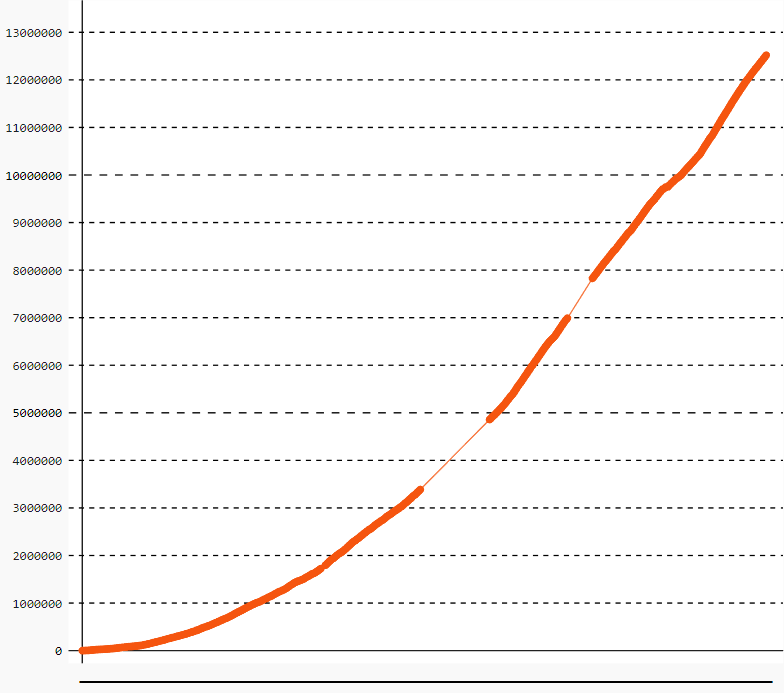
\includegraphics[width=0.5\textwidth]{figures/latest_ids.png}
\caption{A plot showing the latest IDs sent and reported by the simulator. The two thin spots in the line indicate the two times our system was down. The x-axis is the duration of the simulator, and the y-axis is the ID.}
\label{fig:latest_ids}
\end {center}
\end{figure}

The first metrics we set up for monitoring were the number of requests to each of our endpoints using Prometheus. This data collected for monitoring is viewable on the ``/metrics" endpoint. The data is also connected to Grafana and configured with a dashboard. 

We then automated the process of setting up this dashboard when booting up our system. To do this, we downloaded the configuration file of the dashboard as a json, and saved it to the \textbf{Grafana} folder in our repository. As per the way the subsystems interact as described in section 1.3, since Prometheus is added as a data source to Grafana, when booting up our system with the \textit{docker-compose.yml} the Grafana container will point to the configuration file and load Grafana using our downloaded dashboard template.

To improve our ability to be reactive, we used the built-in Prometheus metric ``up" that will track if the system is down, and added the corresponding panel to our dashboard, as shown in Fig. \ref{fig:system_status}. This still requires manually checking the dashboard. Therefore the next step would be to set up an alert to notify the team when the system is down.

\begin{figure}[H]%[!ht]
\begin {center}
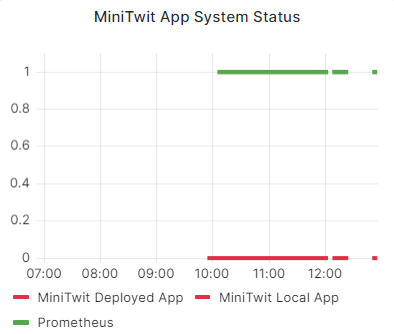
\includegraphics[width=0.5\textwidth]{figures/system_status.png}
\caption{A screenshot showing the panel on our dashboard that shows the system status of our application.}
\label{fig:system_status}
\end {center}
\end{figure}

There are addition metrics we would consider monitoring. We initially monitored the CPU gauge, but did not find the information relevant for our needs at the time. There were a couple of weeks when requests to each endpoint in our system could take many seconds. Therefore we would like to include having a panel displaying a load gauge, indicating the time needed for endpoints to load. For the business perspective we would like to monitor activity level of the app based on users, for example the inflow of users, how often a user tweets, and how users interact with each other.

\subsection{Logging}
% What do you log in your systems and how do you aggregate logs?
% Dee
We set up Grafana Loki to aggregate logs. We had initially installed the Loki plugin within the droplet on DigitalOcean that runs our MiniTwit. Then, in our \textit{docker-compose.yml} we specified the logging driver to be Loki. The first time we ran this we logged into Grafana, connected the Loki data source, and configured a dashboard to display the logs. 

Since our system is built with containers, when releasing a new version of the app and recreating new containers the logs would be lost. By aggregating the logs with Loki we were able to keep logs for analysis even if the containers are deleted or recreated.

Then we automated the process of creating the log dashboard in a similar manner to how we setup the monitoring dashboard. We saved the json containing the log dashboard configuration within \textbf{grafana/dashboards} in our repository. The respective data source configuration was also appended to the automatic.yaml file containing the list of data sources within the Grafana directory.

After switching to Docker Swarm, the logging seems to be broken, therefore this version of our MiniTwit app does not contain logging as of yet.

Further logging...

\subsection{Security Assessment}
% Brief Results of the Security Assessment
% we removed environment credentials from container
% Jakob

We started our security assessment by identifying threats against our website.

\begin{table}[H]
    \centering
    \begin{tabular}{|c|p{6cm}|}
    \hline
        \textbf{Identify Threat sources} & \textbf{Construct Risk scenarios} \\ \hline
        SSH into droplet & Attacker knows IP address, computer name for a droplet, and can add their own private key to gain access.\\ \hline
        SQL injection & Attacker performs SQL injection on web application to download sensitive user data.\\ \hline
        Hacking Digital Ocean account & Attacker using brute force or some other way to hack into our Digital Ocean account, giving them access to our whole application.\\ \hline
        XSS Attack & XSS attack into HTML forms to inject malicious JavaScript\\ \hline
        Connect to PostgreSQL remotely & Attacker uses PSQL to access our stuff.\\ \hline
        Access .env file in webserver container & Hacker accesses the .env file inside the webserver docker container (which contains credentials to the database)\\ \hline
        DDoS attack & Attacker uses a DDoS attack, causing application to shutdown.\\ \hline
    \end{tabular}
    \caption{Identified risks and set up scenarios for each risk }
    \label{tab:my_label}
\end{table}

After identifying the risks, we analysed how big of a deal it would be, if they were to happen. We visualised this with a Risk Matrix.

\subsubsection*{Risk Matrix}

\begin{figure}[H]
\begin{center}
    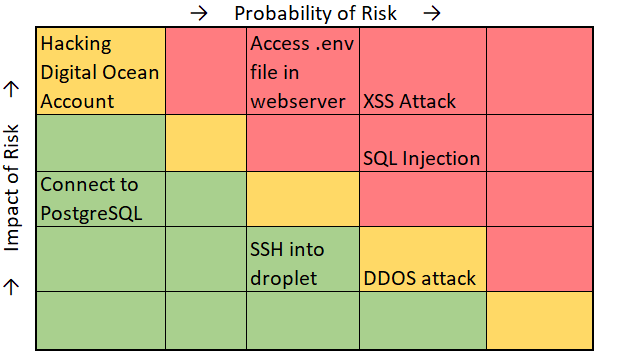
\includegraphics[scale=0.9]{figures/risk assessment.png}
    \caption{Risk Assessment}
  \label{riskmatrix}
\end{center}
\end{figure}

\subsubsection*{Vulnerability scanning}
We used OWASP ZAP to scan our system for vulnerabilities. The results from the scan showed us that we had several threats against our website, including SQL injections and XSS attacks as we had predicted from our analysis.

\subsubsection*{Vulnerability fixing}
A vulnerability from our early analysis, that we decided to get rid of, was the access to our .env files in the web server. 


\subsection{Applied Strategy for Scaling and Load Balancing}
% Adam & sabrina

% \subsubsection*{Docker Swarm}

Scaling and load balancing are newer additions to the system, and are not a part of the development branch / main branch. Auto-scaling is not a feature of the system. Our scaling/load balancing implementation is based off of \href{https://github.com/itu-devops/itu-minitwit-docker-swarm-teraform}{this repository}.

Scaling is done via docker swarm, with which services can easily be replicated across multiple nodes (droplets, in our case) 

\begin{figure}[h]
\centering
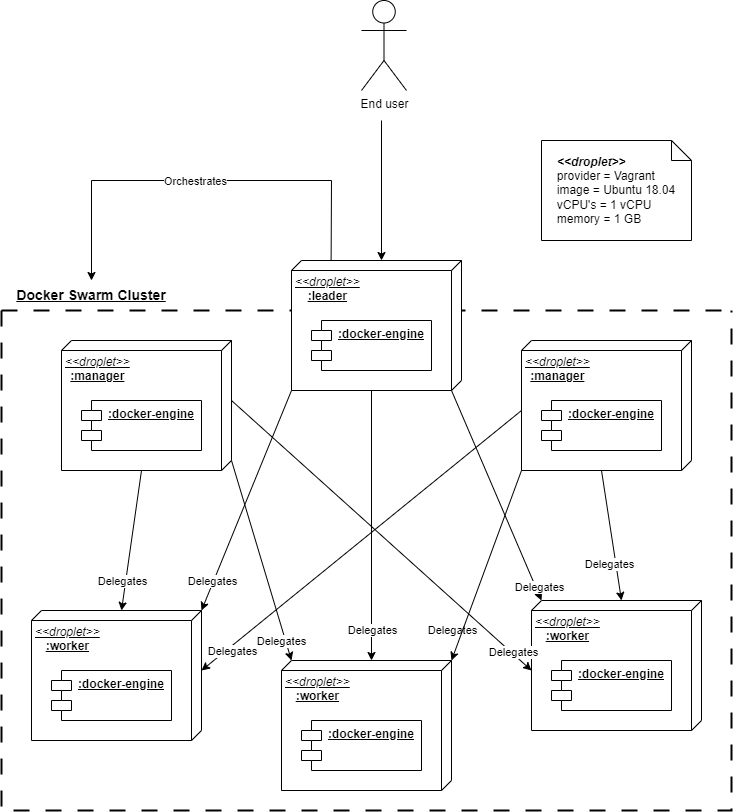
\includegraphics[width=0.8\textwidth]{figures/deploySwarm.png}
\caption{Interactions between nodes in our swarm cluster.}
\label{fig:swarm}
\end{figure}

Each node runs an instance of the docker engine, thus allowing the docker swarm to spread the workload across multiple droplets.

Load-balancing is achieved with nginx configured to route traffic to any of the nodes.

Our default configuration has the minitwit service (see \ref{subsystems}) replicated 9 times, the load balancer replicated 2 times, with the rest of the services only having 1 replica.

There are 3 manager nodes (one of which is a leader), and 3 worker nodes. The manager nodes orchestrate the cluster and delegate work to worker nodes. 


\subsection{Using AI Assistants}
% In case you have used AI-assistants for writing code during your project or to write the report:
% Explain which system(s) you used during the project.
% Reflect how it supported/hindered your process.
% used for our SLA
% tried to use for cookies in the beginning due to lack of documentation. Never made anything with it
% All

Assisted in writing the SLA.

Attempted to use for how to implement ``cookies" using the Gin framework, due to lack of sufficient examples in documentation. We inquired ChatGPT for examples of code, but did not end up using it. So we do not know if this is a good use case.

